\documentclass[11pt,a4paper]{report}
\usepackage[utf8]{inputenc}
\usepackage[ngerman]{babel}
\usepackage[a4paper,left=3cm,right=3cm,top=3cm,bottom=4cm]{geometry}
\usepackage{graphicx}
\usepackage{changepage}
\usepackage{listings}
\lstset{
	language=C++,
	keywordstyle=\color{blue},
    stringstyle=\color{red},
    commentstyle=\color{green},
    morecomment=[l][\color{magenta}]
}
\usepackage{hyperref}
\hypersetup{
	colorlinks=true,
	linkcolor=black,
	filecolor=magenta,
	urlcolor=blue,
}
\usepackage{parskip}
\usepackage{titlesec}
\titlespacing*{\chapter}{0pt}{-50pt}{40pt}

\title{Vulkan - Der Weg zum Dreieck}
\author{Peter Maximilian Kain}
\date{\today}

\begin{document}
\setlength{\parindent}{0em}
\setlength{\parskip}{1em}
\maketitle
\newpage

\tableofcontents
\newpage

\chapter{Einleitung}
Diese Arbeit handelt von Vulkan, der neuesten Grafik-API von der Khronos Group, erschienen im Jahr 2016. Die Khronos Group ist unter anderem bekannt für OpenGL, ebenfalls einer Grafik-API. Vulkan dient nicht als Ersatz für OpenGL, sondern vielmehr als zweite Option. Warum braucht man eine zweite Option?

In OpenGL hatte man zunächst den Immediate Mode, mit dem einem der Großteil der Arbeit abgenommen wurde, man ziemlich schnell entwickeln konnte, aber alles unter einem Einbußen an Performance. Performance ist für Grafikanwendungen jedoch ein äußerst wichtiger Faktor, da sie eine Grenze darstellt, die manche Ideen nicht umsetzbar macht. Mit OpenGL 3.3+, auch als "Modern OpenGL" bezeichnet, wurde diese Performancegrenze angehoben. Man hat mehr Kontrolle über Geschehnisse, die vorher alle im Hintergrund passierten und hat so eine höhere Performance.

Mit Vulkan wurde diese Grenze noch weiter angehoben, aber da Modern OpenGL noch immer brauchbar, und für Entwickler viel einfacher ist, ist Vulkan, wie der Name schon sagt, ein eigenes Produkt. Vulkan soll den Overhead von Modern OpenGL noch weiter reduzieren und so ressourcenschonender und noch performanter sein. Dafür ist die API äußerst verbos und man muss einen Großteil selbst konfigurieren. Der Vorteil dabei ist, dass man als OpenGL Entwickler noch einmal sieht, was denn alles im Hintergrund für einen gemacht wird.
\newpage

\section{Die Vorteile von Vulkan}
Der Hauptkonkurrent zu Vulkan ist momentan Microsoft mit DirectX 12. Um gegen so einen großen Konkurrenten bestehen zu können, braucht es klare Vorteile:

Vulkan ist plattformunabhängiger als DirectX 12. DirectX 12 unterstützt Windows 10 und XBox One X, während Vulkan Windows 7, 8 und 10, Linux, MacOS, Android und iOS untertützt. Auch ist Vulkan im Gegensatz zu DirectX 12 quelloffen. Da ich persönlich auch einen OpenGL Hintergrund habe und mein Projekt auf Linux laufen sollte, war meine Wahl einfach.

\section{Die folgenden Kapitel}
Die folgenden Kapitel sollen Meilensteine am Weg zum ersten Dreieck darstellen. In OpenGL ist das erste Dreieck eine Art Hello World, in Vulkan stellt das Dreieck weit mehr Arbeit dar, jedoch hat man zu dem Zeitpunkt die Idee Vulkans verstanden und das langwierige, aber notwendige Setup hinter einem.

Jedes Beispiel im src Ordner ist ausführbar und beinhaltet so weit wie möglich nur den Code, den man braucht, um das jeweilige Ziel (Name der Datei) zu erfüllen. Die Vorgehensweise ist dabei hauptsächlich übernommen aus dem \href{https://vulkan-tutorial.com}{Vulkan Tutorial}.

\section{Abhängigkeiten}
Die Beispiele haben folgende Abhängigkeiten: \href{https://www.glfw.org/download.html}{GLFW 3.3.2} und \href{https://vulkan.lunarg.com}{Vulkan}. GLFW3 wird hauptsächlich verwendet, um plattformunabhängig Fenster, und spezifisch für Vulkan, einen Surface zu erstellen. In surface.cpp ist die Vorgehensweise der Erstellung von einem Surface als Kommentar verfasst, aber GLFW3 macht einem die Arbeit leichter.

Wozu man Vulkan braucht, sollte selbstverständlich sein. Spezifisch habe ich das Vulkan SDK von LunarG verwendet, weil es empfohlen wird und nicht nur die Notwendigkeiten für Vulkan (Bibliothek und Header), sondern auch Testprogramme und Compiler von GLSL auf SPIR-V (wie später besprochen wird) beinhaltet.

\section{Was wird nicht besprochen}
Diese Arbeit soll keine Dokumentation von Vulkan darstellen (die wäre viel zu umfangreich und im gegebenen Zeitrahmen nicht möglich), sondern vielmehr die Vorgehensweise behandeln, wie man zu den einzelnen Meilensteinen gelangt. Das beinhaltet beispielsweise: Welche Informationen man braucht, um ein Objekt zu erstellen. Jedoch nicht: Eine detaillierte Beschreibung jedes Attributs eines structs, welches man ausfüllen muss, um ein Objekt zu erstellen. Am Ende soll man vor allem den Code halbwegs verstanden haben, der in Form von Beispielen vorliegt:
\newpage
%\newgeometry{left=0.5cm,top=0.5cm,bottom=0.5cm,right=0.5cm}
\begin{adjustwidth}{-2cm}{-2cm}
\begin{center}
	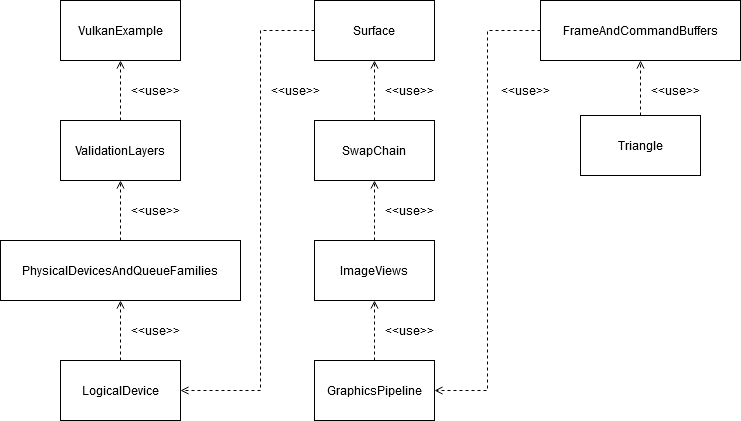
\includegraphics[scale=0.65]{class_dependency_diagram}
\end{center}
\end{adjustwidth}
%\restoregeometry
Diese Beispiele sind alle (fast) aufeinanderfolgend aufbauend (von VulkanExample zu Triangle) und bilden quasi den Weg, den man zum letzten Beispiel, dem Dreieck, beschreiten muss. Der Vorteil an dieser strikten Aufteilung ist es, dass man pro Beispiel nur den Code sieht, den man braucht, um das dem Beispielnamen entsprechende Ziel zu erfüllen.

Das Ziel dieser Arbeit und deren Beispielen ist es, diesen Weg so kurz, aber auch so verständlich wie möglich zu erklären, womit auch gleichzeitig die Beispiele dokumentiert werden.

\chapter{Interagieren mit der Grafikkarte}
Mit Vulkan startet man (fast) von Null. Bevor man mit Rendering beginnen kann, muss man zuerst eine Hardware auswählen, welches man zum Rendern verwenden will (physical device). Das Ziel dieses Kapitels ist es, eine Schnittstelle zu dieser Hardware (logical device) zu erstellen. Man müsste für jedes physische Gerät ein logisches Gerät erstellen, aber Multi-GPU Rendering behandelt dieses Kapitel nicht. Da wir auch nicht in tiefere Gebiete, wie Geometry Shaders, vordringen, ist die einzige Vorraussetzung eine Grafikkarte mit Vulkan Support.\\
Die Abschnitte dieses Kapitels beschreiben die Beispiele:
\begin{enumerate}
	\item vulkan\_example
	\item physical\_devices\_and\_queue\_families
	\item logical\_device
\end{enumerate}

\section{Erstellen einer VkInstance}
Eine VkInstance dient als Initialisierungspunkt von Vulkan, bei dem die Applikation Informationen über sich preisgeben kann. Außerdem dient die Instanz dazu, Informationen über physical devices zu bekommen. Fast alle Vulkan Objekte (gekennzeichnet durch Vk, im Gegensatz zu Funktionen vk) werden durch das Übernehmen von Informationen aus einem struct erstellt (Vk Objektname CreateInfo). So muss man, um eine Instanz zu erstellen, das struct VkInstanceCreateInfo ausfüllen. Um dieses struct zu erstellen, braucht man noch das struct VkApplicationInfo.
Fast alle structs haben in Vulkan das Attribut sType. Dieses dient dazu, ein struct im Low-Level Bereich zu identifizieren und ist daher das erste Attribut in so einem struct. Ein sType ist zwar lang, aber klar definiert: VK\_STRUCTURE\_TYPE\_NAME\_OF\_THE\_STRUCTURE

Für VkApplicationInfo werden wir also VK\_STRUCTURE\_TYPE\_APPLICATION\_INFO angeben.
Ansonsten enthält VkApplicationInfo Informationen über die Applikation, wie der Name, die Version, und die Version der verwendeten Vulkan API. Auch kann man den Namen und die Version einer Engine angeben, die man verwendet. Anhand dieser Informationen kann der Treiber die Applikation optimieren (bspw. man verwendet eine bekannte Engine).

VkInstanceCreateInfo verwendet dieses struct und fügt noch weitere Informationen hinzu, wie die zu verwendeten Validation Layers (besprochen im nächsten Kapitel) und Extensions, die wir benötigen. Vulkan selbst ist wie ein Fundament zu sehen, auf dem man mit Extensions bauen kann. So muss man beispielsweise Extensions hinzufügen, damit Vulkan mit dem Fenster interagieren kann. GLFW3 hat dafür die Funktion glfwGetRequiredInstanceExtensions, welche die notwendigen Extensions zurückliefert, die man dann angeben kann.

Anschließend kann man mit vkCreateInstance die Instanz erstellen. Vulkan bietet einem dabei die Möglichkeit, Callbacks für einen Allocator anzugeben, wenn man denn einen eigenen verwenden möchte. Wir werden das nicht, und geben für so einen Parameter nullptr an. Außerdem liefert eine vkCreate Funktion typischerweise ein VkResult zurück, welches man auf Werte überprüfen kann. Hat es den Wert VK\_SUCCESS, war das Erstellen erfolgreich, jedoch gibt es noch andere Werte, wie z.B.: VK\_ERROR\_OUT\_OF\_HOST\_MEMORY oder VK\_ERROR\_FEATURE\_NOT\_PRESENT. Letzterer Fehler wird im nächsten Abschnitt mehr Sinn ergeben.

\section{Auswählen eines physical device}
Eine Grafikanwendung hat typischerweise Anforderungen an Grafikkarten, wie zum Beispiel, dass die Grafikkarte ein spezielles Feature, wie Geometry Shaders, unterstützt, oder dass die Grafikkarte aufgrund der Rechenleistung dediziert ist. Die Wahl des richtigen physical devices behandelt diese Themen. Mit vkEnumeratePhysicalDevices bekommt man mithilfe der VkInstance die physical devices im System zurückgeliefert. Danach kann man mit vkGetPhysicalDevice(Properties/Features) bestimmte Properties und Features abfragen, die das physical device hat (Beispiel in Execute()). Man könnte dann die Features und Properties gewichten und das Gerät wählen, dass am besten diese Properties und Features unterstützt (im Idealfall alle gebrauchten).

Damit ist man jedoch noch nicht ganz fertig: Man muss auch überprüfen, ob das gewünschte physical device bestimmte Queues hat. Eine VkQueue wird verwendet, um Commands auszuführen (wird später besprochen). Für uns ist momentan wichtig, dass es eine Queue gibt, an die man Commands zum Rendern abgeben kann. Dafür überprüfen wir die Properties der queues auf dem physical device. Diese bekommen wir mithilfe von vkGetPhysicalDeviceQueueFamilyProperties. Die Art der Queue ist im Attribut queueFlags spezifiziert. Wir wollen, dass das VK\_QUEUE\_GRAPHICS\_BIT gesetzt ist, also überprüfen wir das und speichern uns den Index der QueueFamily ab. Nachdem hoffentlich beide Anforderungen erfüllt sind, haben wir unser physical device gewählt! Jetzt müssen wir noch ein logical device erstellen, mit dem Vulkan mit dem physical device interagieren kann.

\section{Erstellen eines logical device}
Bei der Erstellung des VkDevice (logical devices) legt man fest, wieviele Queues man für welche QueueFamilies erstellen will (im Normalfall braucht man nur eine Queue pro QueueFamily), und welche Features und physical device Extensions man verwenden will. Dafür benötigt man die structs VkDeviceQueueCreateInfo und VkDeviceCreateInfo.

In VkDeviceQueueCreateInfo gibt man an, wieviele Queues man für welche QueueFamily mit dem VkDevice erstellen will, sowie die Priority der Queues, welche am Ende das Scheduling betrifft. Für jede QueueFamily muss man so ein struct erstellen.

In VkDeviceCreateInfo gibt man die Adresse zu den VkDeviceQueueCreateInfo structs an, sowie die Anzahl der VkDeviceQueueCreateInfo structs, wie es in C üblich ist. Wenn es nur ein struct ist, wie in diesem Fall, reicht die Adresse zu diesem und 1 für die Anzahl. Des weiteren braucht man die Adresse zu einem VkPhysicalDeviceFeatures struct, der die Information enthält, ob das Feature aktiv, oder nicht aktiv sein soll. Da wir keine besonderen Features verwenden, erstellen wir einen VkPhysicalDeviceFeatures struct, lassen alles mithilfe der Default-Initialization auf VK\_FALSE und geben die Adresse von diesem an. Zu guter Letzt müssen wir noch die Extensions für das physical device angeben. Da wir für das physical device (noch) keine brauchen, lassen wir einfach den count auf 0.

Jetzt können wir mit vkCreateDevice ein logical device erstellen. Die verlangten Queues bekommen wir mit vkGetDeviceQueue. Da geben wir neben dem logical device den Index der QueueFamily an, sowie den Index der Queue (benötigt, wenn man mehr als eine Queue für die QueueFamily angegeben hat, bei uns ist der Index daher 0) und die Adresse einer VkQueue, wo man die Queue speichern will.

Nun haben wir ein logical device und können theoretisch schon anfangen, die Swap Chain zu definieren, jedoch handelt das nächste Kapitel erstmal von einer optionalen Möglichkeit zu Debuggen - den Validation Layers.


\chapter{Validation Layers}
Da Vulkan eine sehr verbose API ist, kann sich bei der Menge an Informationen, die man angeben kann, und muss, leicht ein Fehler einschleichen. Validation Layers dienen dazu, unter anderem solche Fehler aufzudecken und stellen quasi Sicherheitsschichten dar, die man durchdringen muss, damit man zur eigentlichen Funktionalität kommt. Klarerweise kann das nur einen Nachteil haben - Performance. Daher aktiviert man sie generell in einem Debug Build und im Release Build kann man sie ganz einfach nicht aktivieren. Der Vorteil dabei ist, dass man, auch wenn man sie aktiviert, man nur die aktivieren kann, die man braucht. Eine Standard Validation Layer ist VK\_LAYER\_KHRONOS\_validation, welche ich im Laufe dieses Guides verwendet habe. Noch mehr Informationen zu Validation Layers gibt es unter \href{https://gpuopen.com/using-the-vulkan-validation-layers/}{GPU Open}\\
Der Abschnitt dieses Kapitels beschreibt das Beispiel:
\begin{enumerate}
	\item validation\_layers
\end{enumerate}

\section{Hinzufügen von Validation Layers}
Wie wir schon erfahren haben, werden Validation Layers mit dem Erstellen einer VkInstance aktiviert. Das heißt, wir müssen, wie bei den Extensions die Anzahl und Namen der gewünschten Validation Layers im VkInstanceCreateInfo struct angeben. Dazu müssen wir erst einmal wissen, welche Validation Layers es überhaupt gibt. Mit vkEnumerateInstanceLayerProperties kann man diese Information bekommen. Im Sinne dieses Beispiels gibt es auch noch die Methode CheckIfLayerValid, die überprüft, ob die gewünschte Layer vorhanden ist, bevor sie einem Array hinzugefügt wird. Der Array und deren Größe werden dann der CreateInstance Methode vom ersten Beispiel mitgegeben und mit diesen Informationen sind die gewünschten Validation Layers aktiviert.

Will man sich mit diesen ein wenig spielen, enthält die Execute Methode ein kleines Programm, mit dem man verfügbare Layers mit \$PRINT ausgeben kann, Layers hinzufügen kann, und mit \$FINISH zuletzt eine VkInstance mit den angegebenen Layers erstellen kann. Wie schon erwähnt werden wir uns jedoch im weiteren Verlauf mit der Layer VK\_LAYER\_KHRONOS\_validation begnügen.

\chapter{Die Swapchain}
Wer schon Erfahrung mit Grafikprogrammierung hat, der weiß, dass gerenderte Bilder vor der Präsentierung an den Benutzer zuerst in einem Puffer gespeichert werden, wo ein Bild des Puffers nach der Präsentation des angezeigten Bilds getauscht (swap) wird. Der Puffer ist hierfür der Vorteil, dass erstens fertige Bilder präsentiert werden können und nicht On-The-Fly gerendert werden müssen und zweitens, dass der Grafikkarte nicht so schnell langweilig wird. Beispielsweise kann die Grafikkarte nachdem ein Bild gerendert wurde schonmal das nächste Bild rendern, bevor das schon gerenderte Bild überhaupt präsentiert wird.

Diese Puffer sind die Swapchain (ein Puffer ist quasi ein Kettenglied), und diese werden wir in diesem Kapitel konfigurieren und erstellen. Doch bevor wir die Swapchain erstellen, müssen wir erstmal, wie in der Einleitung kurz angesprochen, einen Surface erstellen, der Vulkan quasi als Präsentationsoberfläche dient, also als Weg, mit dem Fenster der Anwendung zu kommunizieren.\\
Die Abschnitte dieses Kapitels beschreiben die Beispiele:
\begin{enumerate}
	\item surface
	\item swap\_chain
\end{enumerate}

\section{Erstellen eines Surface}
Mit GLFW3 ist die Erstellung eines VkSurfaceKHR Objekts einfach. Bevor wir diese Erstellung durchgehen, will ich jedoch die wahrscheinliche Frage beantworten, warum bei VkSurfaceKHR am Ende KHR steht. Dieser Anhang kennzeichnet das VkSurfaceKHR Objekt als Teil einer Extension. Welche Extension? Einer der von glfwGetRequiredInstanceExtensions zurückgelieferten, im speziellen: VK\_KHR\_surface. Wir werden auch später bei der Erstellung der Swapchain diesen Anhang bemerken, da die Swapchain ebenfalls Teil der von GLFW3 verlangten Extensions ist. Nun aber zum Erstellen des Surfaces:

Das Erstellen eines VkSurfaceKHR Objektes wäre standardmäßig nicht plattformunabhängig. Im Fall von Windows müsste vkCreateWin32SurfaceKHR aufgerufen werden, wenn man X11 verwendet, würde die Funktion dafür vkCreateXlibSurfaceKHR heißen. Die Funktionen verlangen beide unterschiedliche structs, die Informationen über das Fenster brauchen (in Windows HINSTANCE und HWND, z.B.). Da GLFW3 für uns schon das plattformunabhängige Erstellen und Verwalten von Fenstern weg abstrahiert, kann es auch ohne Probleme mit einem einzigen Funktionsaufruf ein VkSurfaceKHR Objekt zurückliefern, nämlich mit glfwCreateWindowSurface (benötigt die Instanz, die Adresse zum GLFWwindow, ein Callback für einen Allocator (= nullptr) und die Adresse des VkSurfaceKHR Objekts, das wir erstellen wollen).

Jetzt wäre ein guter Zeitpunkt, den wenigen GLFW3 Code zum Erstellen des GLFWwindow Objektes zu erklären. Der Code dafür ist schon im Beispiel vulkan\_example zu finden und besteht im Ganzen aus 3 Zeilen:
\begin{lstlisting}[language=C++]
glfwWindowHint(GLFW_CLIENT_API, GLFW_NO_API);
glfwWindowHint(GLFW_RESIZABLE, GLFW_FALSE);
glfwWindow = glfwCreateWindow(800, 600, name.c_str(),nullptr,nullptr);
\end{lstlisting}
Auf die erste und zweite Zeile kommen wir später noch zurück. Die dritte Zeile betrifft das Erstellen eines GLFWwindow Objekts. Die wichtigen Parameter sind hierfür Breite/Höhe des Fensters, sowie der Titel. Der loop zum Offenhalten des Fensters sieht folgendermaßen aus:
\begin{lstlisting}[language=C++]
while (!glfwWindowShouldClose(glfwWindow)) {
	glfwPollEvents();
}
\end{lstlisting}
Der Code ist ziemlich selbsterklärend. Solange das Fenster nicht geschlossen werden soll (also kein Close-Event), dann halte nach Events ausschau (wie z.B. einem Close-Event). Normalerweise müsste man auch glfwSwapBuffers aufrufen und das ist der Zeitpunkt, wo wir die ersten beiden Zeilen von oben besprechen können: Die erste Zeile macht das Aufrufen von glfwSwapBuffers zu einem Fehler. Wir erstellen ja mit Vulkan unsere eigene Swapchain, die das Swappen von Image Buffers übernimmt. Die zweite Zeile verhindert einfach das Ändern der Größe des Fensters. Wenn das Fenster, und somit der Surface verändert werden würde, müsste man nämlich die Swapchain neu erstellen, da die derzeit gespeicherten Informationen ungültig wären (dazu später mehr).

Nun, da wir den GLFW3 Code besprochen hätten, zurück zur Erstellung des Surfaces - wir sind nämlich noch nicht fertig. Unsere Anforderungen an das physical device haben sich geändert! Das physical device muss erst einmal auch Surfaces unterstützen! Also passen wir den Code für die Erstellung von physical und logical devices noch einmal an und überprüfen den Support für Surfaces in den QueueFamilies. Es sollte nämlich eine Queue geben, die letztendlich mit unserer Swapchain interagiert und ihr die gerenderten Bilder zukommen lässt. Das können wir mit der Funktion vkGetPhysicalDeviceSurfaceSupportKHR überprüfen. Diese erwartet sich das physical device, den QueueFamilyIndex, unser VkSurfaceKHR Objekt und einen VkBool32 output, der das Ergebnis beinhaltet.

Diesen Code können wir zu dem hinzufügen, der überprüft, ob das jeweilige physical device eine rendering Queue hat, also zu den physical device checks. Beim Erstellen des logical devices müssen wir auch beachten, dass es nun eine zweite QueueFamily gibt und noch ein VkDeviceQueueCreateInfo struct für diese QueueFamily hinzufügen (wir wollen wieder nur eine Queue erstellen). Klarerweise müssen wir auch den VkDeviceCreateInfo struct anpassen, da wir zwei VkDeviceQueueCreateInfo structs haben, die wir angeben müssen. Zu guter Letzt noch ein Aufruf von vkGetDeviceQueue um die neue Queue zu speichern und - das wars!

\section{Erstellen der Swapchain}
Um überhaupt eine Swapchain erstellen zu können, müssen wir erstmal eine weitere Extension hinzufügen. Warum ist diese Extension nicht Teil der von GLFW3 verlangten Extensions? Ich vermute mal, weil die Erstellung der Swapchain nicht mehr im Anwendungsgebiet von GLFW3 liegt. Und in Vulkan ist das Konzept "You get what you pay for" ja allgegenwärtig.

Aber wie hieß noch schnell die Extension genau? Da kann uns Vulkan aushelfen, und zwar ist ein Makro VK\_KHR\_SWAPCHAIN\_EXTENSION\_NAME definiert. Wir müssen also nur wissen, dass VkSwapchainKHR KHR als Anhang hat und Swapchain heißt. Das bringt auf ersten Blick nicht viel, wenn man weiß, dass die Extension "VK\_KHR\_swapchain" heißt, aber immerhin kann man sich mit dem Makro sicher sein, dass man es richtig geschrieben hat. Wie fügen wir jetzt die Extension hinzu? Mit dem Erstellen eines logical devices natürlich! Wir sollten vorher noch sicherstellen, dass das physical device diese Extension unterstützt, also wieder den Code modifizieren, der die physical devices überprüft und schauen, dass alle benötigten Extensions in den verfügbaren Extensions vorkommen. Wie bekommt man nochmal alle verfügbaren Extensions? Mit vkEnumerateDeviceExtensionProperties.

Nun, da wir diesen Schritt erledigt haben, können wir die Swapchain erstellen. Jedoch brauchen wir noch Informationen: Wir wissen ja nicht, welche Optionen zum Konfigurieren der Swapchain überhaupt unterstützt werden! Wir müssen 3 Dinge überprüfen: Was unser Surface so unterstützt - VkSurfaceCapabilitiesKHR, dann welches Farbformat und Farbbereich unterstützt wird - VkSurfaceFormatKHR, und zuletzt, wie Bilder in der Swapchain angezeigt werden können - VkPresentModeKHR. Diese Informationen lassen sich mithilfe von vkGetPhysicalDeviceSurface(Capabilities/Formats/PresentModes)KHR bekommen und sind bei mir, wie auch im \href{https://vulkan-tutorial.com}{Vulkan Tutorial}, zusammen in einem struct gespeichert. Nun müssen wir aus den verfügbaren Optionen wählen, also die Swapchain konfigurieren. Dazu braucht man unter anderem die 3 Objekte VkSurfaceFormatKHR, VkPresentModeKHR und VkExtent2D.

Vulkan lässt einem sehr viele Optionen, aber normalerweise kann man sich an ein paar festhalten: Beispielsweise sind 8-Bit RGBA Kanäle, sowie das SRGB Format nicht verkehrt. Also gehen wir, wie bei fast jeder Konfiguration, alle verfügbaren Optionen (VkSurfaceFormatKHR) durch und wählen uns ein VkSurfaceFormatKHR Objekt aus, wo das .format Attribut den Wert VK\_FORMAT\_B8G8R8A8\_SRGB, und das .colorSpace Attribut den Wert VK\_COLOR\_SPACE\_SRGB\_NONLINEAR\_KHR hat. Wenn uns diese zwei Dinge komplett egal sind, oder es diese Optionen nicht gibt, kann man immer das Format so konfigurieren, dass man einfach das erste verfügbare Format nimmt.

Haben wir uns das gewünschte VkSurfaceFormatKHR Objekt gespeichert, können wir zum Beispiel mit VkPresentModeKHR weitermachen. Mit diesem Objekt wird bestimmt, wann ein Bild dem User Präsentiert wird. Garantiert verfügbar ist der Modus VK\_PRESENT\_MODE\_FIFO\_KHR, der aussagt, dass die Swapchain eine Queue ist. Die Bilder kommen vorn auf den Bildschirm und werden von hinten von der Grafikkarte nachgefüllt. Ist diese Queue voll, muss die Grafikkarte warten. Das ist natürlich nicht optimal, da wir ja unsere Rechenleistung bestmöglich ausnützen wollen. Deshalb überprüfen wir, ob es nicht den PresentMode VK\_PRESENT\_MODE\_MAILBOX\_KHR gibt. Da müsste die Grafikkarte nicht mehr warten, sondern überschreibt einfach die Bilder in der Queue mit neu gerenderten. Wenn es diesen Modus nicht gibt, geben wir uns aber auch mit dem ersten zufrieden.

Zu guter Letzt brauchen wir noch ein Objekt: Ein VkExtent2D Objekt, das in dem Fall als Auflösung der Bilder in der Swapchain dient. Dazu brauchen wir das VkSurfaceCapabilitiesKHR Objekt. Dieses Objekt beinhaltet folgende Informationen über den Extent: .(max/min)ImageExtent und .currentExtent. Generell speichert man sich einfach den .currentExtent, aber es kann sein, dass im .currentExtent die Dimensionen den Maximalwert von einem 32-Bit unsigned Integer annehmen. In diesem Fall müssen (und können) wir den Extent selbst bestimmen, werden dabei aber durch .(max/min)ImageExtent beschränkt. Wir lösen das so, dass wir uns von GLFW3 mithilfe von glfwGetWindowSize die Größe des Fensters mitteilen lassen und sicherstellen, dass die Breite und Höhe nicht über .(max/min)ImageExtent hinausragt. So können wir selbst ein VkExtent2D Objekt erstellen, indem wir .width und .height setzen und dieses abspeichern.

Jetzt heißt es wieder: Ein struct mit diesen Informationen ausfüllen. In dem Fall benötigen wir das struct VkSwapchainCreateInfoKHR. Dieses struct ist sehr groß und benötigt viele Informationen. Um das struct ganz ausfüllen zu können müssen wir uns noch Gedanken darüber machen, wieviele Bilder (=Puffer) wir denn in unserer Swapchain haben wollen. Das VkSurfaceCapabilitiesKHR beinhaltet jedenfalls schon einmal einen .(max/min)ImageCount. Wir könnten uns mit dem .minImageCount zufrieden geben, aber generell wird empfohlen, mindestens ein Bild mehr zu haben als der .minImageCount. Allerdings dürfen wir nicht mehr als der .maxImageCount verlangen. Ist dieser gleich 0 ist jedoch kein Maximum vorgegeben.

Nachdem wir dies sichergestellt haben, können wir anfangen, VkSwapchainCreateInfoKHR zu befüllen. Neben unserem VkSurfaceKHR Objekt und den ausgesuchten PresentModes usw. benötigt der struct weitere Informationen, wie die Schichten eines Bildes, wenn wir beispielsweise 3D Bilder rendern wollen, oder die imageUsage. Man kann direkt in die Swapchain rendern (in dem Fall auf VK\_IMAGE\_USAGE\_COLOR\_ATTACHMENT\_BIT setzen), oder, wenn man das Bild nach dem Rendern bearbeiten möchte (Post Processing), dieses später hinzufügen (VK\_IMAGE\_USAGE\_TRANSFER\_DST\_BIT).

Wenn unsere QueueFamilies für Graphics und Presentation nicht die gleichen sind, müssen wir den Zugriff auf Bilder der Swapchain definieren. Wir wollen ja mit einer Queue die Bilder rendern und mit einer anderen Queue die Bilder der Swapchain zukommen lassen. Haben diese beiden Queues nicht dieselbe QueueFamily, kommt das zu Konflikten. Deshalb kann man zwischen VK\_SHARING\_MODE\_(CONCURRENT/EXCLUSIVE) wählen, sowie die Anzahl der queueFamilies und deren Indices angeben. Schließlich kann man, wenn man möchte, noch Transformationen vor dem Anzeigen angeben, sowie angeben, ob das Fenster anhand des Alphakanals durchsichtig sein soll (wie man zum Beispiel beim Linux Terminal einstellen kann), und, ob die Pixel, die sich beispielsweise hinter einem anderen Fenster befinden, uns egal sind, oder nicht (ersteres führt klarerweise zu besserer Performance).

Jetzt bleibt uns nur noch ein Feld übrig: .oldSwapchain. Ich habe schonmal erwähnt, dass die Swapchain z.B. beim Vergrößern des Fensters z.B. ungültig werden kann. In dem Fall muss man sie neu erstellen, und die alte Swapchain bei dem Feld angeben. Da wir unsere erste Swapchain erstellen, befassen wir uns nicht damit und geben VK\_NULL\_HANDLE an.

Fast zwei Seiten später können wir endlich ein VkSwapchainKHR Objekt mittels vkCreateSwapchainKHR erstellen, und Zugriff auf die Bilder der Swapchain für das spätere Rendering mittels vkGetSwapchainImagesKHR bekommen.

\chapter{Die Grafikpipeline}
Die Grafikpipeline ist wohl der größte Brocken an Konfiguration in Vulkan. Ich werde versuchen, in diesem Kapitel eher oberflächlich zu bleiben, um es nicht unnötig lang zu machen. Die Grundsätze von Vulkan haben wir mittlerweile verstanden. Es sind wieder einmal structs auszufüllen, und zwar sehr viele structs. Die Grafikpipeline selbst beschreibt die Schritte, wie man von rohen Daten zu einem Bild am Bildschirm kommt. Wir werden in diesem Kapitel auch mit Shadern arbeiten. Shader sind Programme, die auf der Grafikkarte laufen und werden üblicherweise von Menschen geschrieben, sind also programmierbar. Neben programmierbaren Schritten in der Grafikpipeline gibt es auch nicht programmierbare. Dazu zählen die Schritte Input Assembler, Rasterization und Color Blending. Diese kann man nicht programmieren, aber konfigurieren. Die einzigen, wirklich optionalen, Schritte sind Tessellation Shader und Geometry Shader. Diese braucht man für spezielle Techniken in 3D Grafik, wie zum Beispiel Fell simulieren mithilfe von Geometry Shadern oder für Objekte mit "Tiefe", wie zum Beispiel eine Ziegelsteintextur auf einer flachen Wand realistisch aussehen zu lassen, mithilfe von Tessellation Shadern.

Wir werden uns daher "nur" mit Vertex und Fragment Shadern auseinandersetzen. Ein Vertex Shader übernimmt und transformiert die Eckpunkte, die er von der Input Assembler Schicht bekommen hat, und ein Fragment Shader bestimmt die Farbe der zurückgelieferten Pixel der Rasterization Schicht. Fragment Shader können sehr komplex sein und beinhalten die meisten Effekte, wie zum Beispiel Nebel oder Beleuchtung. Ich habe die Shader in GLSL verfasst, der OpenGL Shading Language, man kann jedoch Shader für Vulkan in allen unterstützten Sprachen schreiben, da diese mithilfe eines Compilers auf ein Format, nämlich dem Bytecode SPIR-V, gebracht werden. Für GLSL gibt es unter anderem das im LunarG SDK existierende Programm glslc, welches von Google entwickelt wurde und ich verwendet habe. Diese Arbeit soll natürlich kein GLSL Tutorial sein, aber es ist wichtig, zu verstehen, was genau passiert:

Im Vertex Shader (data/triangle\_vs.glsl) ist es wichtig, zu verstehen, dass wir eigentlich eine Schicht der Grafikpipeline auslassen. Die Eckpunkte sind dabei im Vertex Shader definiert, und nicht, wie üblich, in einem Vertex Buffer. Das liegt einfach daran, dass man den Vertex Buffer wieder einmal selbst erstellen muss, und, da man das so umgehen kann, das ein schnellerer Weg zum ersten Dreieck ist. Das wird Auswirkungen auf unsere Konfiguration der Grafikpipeline haben, wie wir später sehen werden. Jeder Shader in GLSL hat, wegen des Einflusses der Programmiersprache C, auch eine main Funktion, die wir später als Einstiegspunkt definieren werden.

Im Vertex Shader, der für jeden Vertex (Eckpunkt) ausgeführt wird, definieren wir die gl\_Position des Vertex. Dabei bedienen wir uns der Variable gl\_VertexIndex, die den Index des jetzigen Vertex darstellt. Das passt perfekt zur Indizierung des Arrays. Der Datentyp "vec" steht dabei klarerweise für "Vektor".

Im Fragment Shader tut sich zu viel für ein Tutorial, da hab ich mich ein wenig gespielt. Wenn wir jedoch alles ignorieren: Was müssen wir im Fragment Shader angeben? Die Farbe des Pixels. Der Fragment Shader wird für jeden Pixel (der von der Rasterization Schicht für die Vertices zurückgeliefert wurde) ausgeführt. Da kommt die hohe Nebenläufigkeit der Grafikkarte ins Spiel (da das der Fall ist, hat kein Shader des Pixels 123 Informationen über den Shader des Pixels 124 z.B, Shader sind also voneinander abgeschottet). Um zum Output des Fragment Shaders zurückzukommen: Wir müssen in der main Funktion angeben, welche Farbe der Pixel haben soll. Das geht einfach, indem wir eine als Output angeben und deren Wert in main setzen. Das ist einfach ein vec4 mit rgba von 0.0 bis 1.0 statt 0 bis 255. Bei rot hätten wir also "farbe = vec4(1.0, 0.0, 0.0, 1.0)". Weiters sehen wir "layout(location = 0)". Das wird uns schon bald mehr sagen. Mehr Informationen zu Fragment Shadern und deren Möglichkeiten finden sich im exzellenten \href{https://thebookofshaders.com/}{Book of Shaders}\\
Der Abschnitt dieses Kapitels beschreibt das Beispiel:
\begin{enumerate}
	\item{graphics\_pipeline}
\end{enumerate}

\section{Erstellen der Grafikpipeline}
\subsection{Erstellen eines RenderPass Objekts}
Ein RenderPass ist quasi eine Sammlung von Attachments, Subpasses und Dependencies zwischen Subpasses. Dependencies sind zum synchronisieren von zwei Subpasses zuständig. Attachments werden von Subpasses verwendet. Das Color Attachment, welches wir verwenden, sagt zum Beispiel unter Anderem aus, was beim Lesen und Schreiben des Images des Swapchain passieren soll. Wenn wir es lesen, wollen wir es beispielsweise erst Clearen ("Löschen", mit einer Farbe überschreiben). Wenn wir es wieder zurück schreiben wollen wir es speichern. Dafür gibt es auch mehrere andere Optionen. Einen Subpass ist quasi ein Rendervorgang.

Es gibt die structs VkAttachmentDescription, quasi die eigentlichen Attachments, VkAttachmentReference, eine Referenz auf das Attachment, welche an das nächste struct, VkSubpassDescription weitergegeben werden kann. VkSubpassDescription beschreibt einfach den Subpass. Dann gibt es noch VkSubpassDependency, welche die dependency zwischen Subpasses beschreibt. Diese drei structs (VkAttachmentDescription, VkSubpassDescription und VkSubpassDependency) gibt man beim struct VkRenderPassCreateInfo an, welches zum Erstellen eines RenderPass Objekts mittels vkCreateRenderPass gebraucht wird.

\subsection{Erstellen der restlichen Grafikpipeline}
Nachdem wir uns so kurz wie möglich mit RenderPasses beschäftigt haben, können wir uns jetzt auf die eigentliche Grafikpipeline konzentrieren. Die Methode "CreateGraphicsPipeline" beginnt damit, die Shader zu laden. Dabei geben wir mit "main" auch den Einstiegspunkt an. Ich habe für das Laden der Shader auch eine eigene Klasse definiert, damit wir einen Destruktor haben. Diese ShaderModules werden am Ende der Funktion nämlich nicht mehr gebraucht. Danach folgt eine Menge an Schritten, die in Funktionen aufgeteilt sind. Das ist so geplant, dass man die Funktionen quasi als Module sieht, die man auch austauschen kann, sollte man eine andere Funktionalität benötigen, so wie es bei den Beispielen mit dem Überprüfen des physical devices ist, wenn man sich den Code schon mal genauer angeschaut hat. Die Default Funktionen sind alle am Ende der Datei zu finden. Man bedenke noch einmal, dass wir es nicht mehr mit programmierbaren Schichten der Grafikpipeline zu tun haben, sondern nur noch konfigurieren können. So füllt jede Funktion ein oder mehrere struct und liefert diese zurück.

Wir werden jede der Funktionen kurz durchgehen:
\begin{enumerate}
	\item setupVertexBuffer()
	\item setupInputAssembly()
	\item setupViewportScissorInfo()
	\item setupViewport()
	\item setupRasterizer()
	\item setupMultisampling()
	\item setupColorBlendAttachment()
	\item setupColorBlending()
	\item setupPipelineLayout()
\end{enumerate}

\subsubsection{setupVertexBuffer}
Liefert ein VkPipelineVertexInputStateCreateInfo struct\\
Diese Funktion würde den VertexBuffer beschreiben, den wir normalerweise verwenden würden, wie zum Beispiel, der Typ (und somit die Größe) von Vertex Data (Wir können nicht nur Positionen mitgeben, sondern zum Beispiel auch Farben pro Vertex (werden dann interpoliert), oder, wenn man sich mit Texturen beschäftigt, wird man auch Texture Koordinaten brauchen. Die Größe von den gesamten Daten, sowie von den einzelnen Daten ist somit äußerst wichtig). Da wir in dem Fall keinen Vertex Buffer verwenden, gibt es auch nichts zu beschreiben.

\subsubsection{setupInputAssembly}
Liefert ein VkPipelineInputAssemblyStateCreateInfo struct\\
Ganz überspringen können wir diese Schicht trotzdem nicht, denn sie enthält Informationen, wie die Eckpunkte interpretiert werden sollen. Wir haben uns dazu entschieden, dass jeweils drei Eckpunkte ein Dreieck definieren, man könnte aber auch zum Beispiel jeden Eckpunkt als Punkt sehen, oder jeweils zwei als Linie. Das wird hier angegeben.

\subsubsection{setupViewportScissorInfo}
Liefert ein VkViewport struct und ein VkRect2D struct\\
Die zurückgelieferten Daten dieser Funktion werden von der nächsten verwendet. Sie benötigt außerdem ein VkExtent2D Objekt (wir können einfach das von der Swapchain angeben). Diese Funktion beschreibt die Größe des Bereiches, in den wir rendern wollen. Der Viewport ist dabei der Bereich, in dem ein Bild angezeigt wird, die Scissor ist der Bereich des Viewports, der angezeigt wird. Dabei hängt die Scissor nicht vom Viewport ab. Deckt also die Scissor den Viewport ab, jedoch nicht die gesamte Fläche des Fensters, wird trotzdem alles vom Viewport gezeichnet werden. Zur Konfiguration gibt man einfach die vier Punkte eines Rechtecks an, welches diese Objekte darstellt und begrenzt. Zusätzlich hat der Viewport noch eine .(max/min)Depth für die Z-Koordinate von 3D Szenen.

\subsubsection{setupViewport}
Liefert ein VkPipelineViewportStateCreateInfo struct\\
Hier werden einfach die beiden structs aus der vorigen Funktion angegeben. Nicht mehr. Nicht weniger.

\subsubsection{setupRasterizer}
Liefert ein VkPipelineRasterizationStateCreateInfo struct\\
Hier werden Informationen angegeben, wie Informationen über die Art der Rasterization, die man haben will: Will man zum Beispiel eine Fläche gefüllt, oder nur die Linien zwischen Eckpunkten (Wireframe)? Wir wollen in dem Fall eine gefüllte Fläche. Eine wichtige Konfiguration ist noch Culling. Culling ist das "weglassen" von unnötiger Information. Ein 3D Objekt, zum Beispiel: Wir haben eine zweidimensionale Fläche zum Rendern. Man kann sich das wie ein Foto eines 3D Objektes vorstellen. Man sieht nur einen Teil, der Rest ist verdeckt. Dieser verdeckte Rest muss nicht unbedingt gezeichnet werden. Das bringt ein Plus an Performance. Wir müssen nur angeben, ob wir den vorderen (nicht verdeckten) oder den hinteren (verdeckten) Teil cullen wollen und müssen noch definieren, was denn ein vorderer Teil ist.

Das geschieht anhand der Reihenfolge der Eckpunkte. In unserem Fall: Wenn die Eckpunkte im Uhrzeigersinn gezeichnet werden, ist die Fläche der Vorderteil des Objektes und wird (in unserem Fall) also nicht gecullt. Stellt man sich jetzt vor, man begibt sich hinter das Object, so sind die Eckpunkte nicht mehr im Uhrzeigersinn gezeichnet, sondern gegen den Uhrzeigersinn gezeichnet (Leicht mit dem Dreieck vorstellbar). Das heißt, wir befinden uns vor der Rückseite des Objektes. Das Dreieck würden wir mittlerweile nicht sehen, das wird gerade "weggecullt".

\subsubsection{setupMultisampling}
Liefert ein VkPipelineMultisampleStateCreateInfo struct\\
Benötigt man nicht unbedingt, dient zur Kantenglättung. Wenn man es aktivieren möchte, ist das ein eigenes physical device Feature. Da wir es nicht brauchen, tut sich hier nicht viel.

\subsubsection{setupColorBlendAttachment}
Liefert ein VkPipelineColorBlendAttachmentState struct\\
Dieses struct brauchen wir für die Color Blending Schicht. Color Blending passiert, wenn die Farbe, die ein Fragment Shader für einen Pixel zurückliefert mit einer schon vorhandenen Farbe des Pixels kombiniert werden muss. Den Blendvorgang kann man dabei ziemlich frei konfigurieren, es gibt verschiedene Arten, die beiden Farben zu mischen. Für ein simples Dreieck braucht man diese Mischvorgänge in dieser komplexen Form nicht, so deaktivieren wir sie und sorgen einfach dafür, dass die Farbe eines Pixels des Bilds mit der vom Fragment Shader zurückgelieferten Farbe überschrieben wird. Damit dies jedem der rgba Farbkanäle passiert, geben wir eine .colorWriteMask an.

\subsubsection{setupColorBlending}
Liefert ein VkPipelineColorBlendStateCreateInfo struct\\
In dieser Funktion geben wir die Anzahl der ColorBlendAttachments der vorigen Funktion (in unserem Fall nur eines), sowie die ColorBlendAttachments selbst an.

\subsubsection{setupPipelineLayout}
Liefert ein VkPipelineLayoutCreateInfo struct\\
Ein Pipeline Layout würde man brauchen, wenn man z.B. uniform Werte in Shadern verwendet. Uniform Werte können laufend von Programm aktualisiert werden. Beispiele dafür sind z.B. Zeit (Für Animationen oder Farben in Shadern), oder, wenn man sich später mit Texturen beschäftigt, für Texturen, die man im Hauptprogramm lädt und dann an die Grafikkarte sendet (sampler2D). Da wir das alles für ein Dreieck nicht brauchen, ist diese Funktion wiederum ziemlich verständlich gehalten.

\subsubsection{Rückblick}
Wir sehen also, obwohl wir nicht alle Schichten benötigen, verlangt Vulkan trotzdem ein explizites Setup der Grafikpipeline. Nachdem wir alle Informationen beisammen haben, besteht das Erstellen der Pipeline nur noch aus simplen Zuweisungen.

\subsubsection{Das Finale}
Zum Schluss müssen wir nur noch zwei Objekte erstellen: Einmal das VkPipelineLayout und einmal die VkPipeline selbst. Ersteres kann man mit vkCreatePipelineLayout erstellen, da wir ja schon ein VkPipelineLayoutCreateInfo befüllt haben. Bevor wir das zweite Objekt mit vkCreateGraphicsPipelines erstellen können, müssen wir noch ein VkGraphicsPipelineCreateInfo struct füllen.

Erst einmal kehren wir zu den Shadern zurück. Wir haben für jeden Shader ein ShaderModule erstellt, müssen aber noch den Einstiegspunkt und den Typ des Shaders, also Vertex oder Fragment Shader angeben. Das können wir in VkPipelineShaderStageCreateInfo structs ausfüllen. Dafür habe ich eine Funktion im vulkan\_helper header geschrieben, die für uns so ein struct ausfüllt. Da wir für jeden Shader diese Informationen angeben müssen, haben wir also zwei VkPipelineShaderStageCreateInfo structs. Diese geben wir zusammen mit der Anzahl dem VkGraphicsPipelineCreateInfo struct weiter. Der Rest ist zum Ausfüllen mit unseren bereits bestehenden structs. Das Attribut .subpass gibt den Index der Subpasses an, für den die Graphics Pipeline verwendet wird. Da wir nur einen subpass haben, geben wir als Index 0 an. Vulkan bietet einem außerdem die Möglichkeit, eine GraphicsPipeline mithilfe einer bereits bestehenden GraphicsPipeline zu erstellen, wenn die beiden Pipelines beispielsweise viel Gemeinsamkeiten haben. Dafür sind die beiden letzten Attribute da, die wir aber nicht verwenden müssen. 
Nach einem abschließenden Aufruf von vkCreateGraphicsPipelines haben wir unsere GraphicsPipeline erstellt und sind damit fast am Ende unserer Reise zum Dreieck.

\chapter{Frame- und Commandbuffers}
Das Letzte, was uns noch am Zeichnen des Dreiecks, oder irgendwelchen 2D Objekten, hindert, sind Framebuffer und Commandbuffer. Wir haben oft davon geredet, dass wir ein Bild in der Swapchain verändern wollen. Die eigentlichen Rendertargets sind dabei immer Framebuffer. Wir müssen also Framebuffer erstellen, die wir den Bildern in der Swapchain zuweisen können. In Vulkan werden Renderfunktionen nicht direkt aufgerufen, sondern in einem Commandbuffer im Vorhinein aufgezeichnet. Diese Commandbuffer kann man dann an Queues weitergeben, wo die aufgezeichneten Operationen dann durchgeführt werden.\\
Die Abschnitte dieses Kapitels beschreiben die Beispiele:
\begin{enumerate}
	\item{image\_views}
	\item{frame\_and\_command\_buffers}
\end{enumerate}

\section{Erstellen von Image Views}
Image Views wurden in meiner Hierarchie schon vor der Grafikpipeline erstellt, jedoch kann man sie in diesem Kapitel besser erklären. Image Views sind der erste Schritt zum Erstellen von Framebuffers. Wie der Name schon sagt, beschreiben sie eine bestimmte "Sicht" auf Bilder. Die Bilder, auf die wir zugreifen wollen, sind die Bilder der Swapchain (Nochmal zur Auffrischung: ...die wir in einem vector mithilfe von vkGetSwapchainImagesKHR gespeichert haben). Wir müssen also pro Swapchain Image ein Image View erstellen, also werden wir die Image Views wieder in einem vector speichern. Pro Image View müssen wir, bevor wir es mit vkCreateImageView erstellen, einen struct, VkImageViewCreateInfo ausfüllen. Das erste wichtige Attribut ist der .viewType. Wir wollen zwar keine Sicht auf Texturen, aber es gibt trotzdem die Möglichkeit auf 1D/2D/3D Texturen, sowie Cube Maps zuzugreifen. Wenn wir auf einer Textur zeichnen wollten, würden wir wohl eine 2D Textur nehmen, also tun wir das auch. Da wir auf Bilder der Swapchain zugreifen, werden wir auch nicht die Möglichkeiten der nächsten Attribute außergewöhnlich ausnutzen. Das Format wird das Format der Swapchain bleiben, wir wollen auch nicht die rgba Kanäle ändern. Wenn die Images der Swapchain 3D wären, und wir somit mehr als einen Layer angegeben hätten, könnten wir Image Views auf unterschiedliche Layer eines Swapchain Images erstellen und somit auf die einzelnen Layers zugreifen. Für uns ist das aber unwichtig. Nachdem wir den struct ausgefüllt haben, aktualisieren wir in einem for loop, welcher die Swapchain Images durchgeht immer das .image Attribut, auf das sich das Image View bezieht. Danach können wir im loop die Image Views mit vkCreateImageView direkt im vector erstellen.

\section{Erstellen von Frame- und Commandbuffers}
\subsection{Erstellen von Framebuffers}
Da wir gerade eben Image Views besprochen haben, werde ich mit Framebuffers fortsetzen. Framebuffers sind ähnlich einfach zu erstellen wie Image Views. Wiederum werden wir pro Image View einen Framebuffer erstellen, also wieder in einem vector abspeichern. Das Erstellen eines Framebuffer erfolgt mit vkCreateFramebuffer. Was werden wir noch brauchen? Richtig - wir müssen wieder ein CreateInfo struct ausfüllen, nämlich VkFramebufferCreateInfo. Zuerst müssen wir angeben, welcher RenderPass diesen Framebuffer verwenden soll. Dann die Attachments und deren Anzahl, die in unserem Fall eins beträgt und das Image View ist. Es folgt die Breite und Höhe des Framebuffers, wo wir einfach die Extent von der Swapchain verwenden, damit dieser gleich groß wie ein Swapchain Image ist. Und wiederum hat der Framebuffer nur eine Layer. Nun sind wir mit dem Ausfüllen fertig und können pro Image View vkCreateFramebuffer aufrufen.

\subsection{Erstellen von Commandbuffers}
Das Erstellen von Commandbuffers besteht aus drei Schritten: Command Pool erstellen, Commandbuffer erstellen, Operationen aufzeichnen.

\subsubsection{Erstellen eines Command Pools}
Command Pools dienen zum Verwalten von Commandbuffers. Das Erstellen eines Command Pools ist dabei sehr einfach: Wir müssen nur eine QueueFamily angeben, für die die Commandbuffer, die wir dem Command Pool hinzufügen gedacht sind. Da wir ein Dreieck zeichnen wollen, entscheiden wir uns für die graphicsFamily. Das müssen wir im VkCommandPoolCreateInfo struct bekanntgeben, bevor wir vkCreateCommandPool aufrufen.

\subsubsection{Erstellen eines Commandbuffers}
Wieder müssen wir pro Framebuffer einen Commandbuffer erstellen. Warum? Werden wir verstehen, wenn wir Operationen aufzeichnen. Fürs erste gibt es das VkCommandBufferAllocateInfo struct zu füllen, womit wir alle Commandbuffers auf einmal erstellen werden. Wir müssen nur das Command Pool angeben, das die Commandbuffer verwalten soll, wieviele Commandbuffer wir erstellen wollen und, ob es primäre oder sekundäre Commandbuffer sein sollen. Was ist der Unterschied? Primäre Commandbuffer können in eine Queue submitted werden, aber nicht von anderen Commandbuffers aufgerufen werden. Bei sekundären Commandbuffers ist das genau das Gegenteil. Warum soll man einen Commandbuffer aufrufen wollen? Zur Wiederverwendung zum Beispiel. Pro Commandbuffer erstellen wir ja Quasi eine Prozedur.

Nachdem wir also angegeben haben, dass wir primäre Commandbuffer wollen (schließlich wollen wir sie an eine Queue übergeben), können wir mit vkAllocateCommandBuffers Commandbuffer erstellen. Somit bleibt nur noch das Aufzeichnen von Operationen.

\subsubsection{Aufzeichnen von Operationen}
Zuerst müssen wir die Commandbuffer auf das Aufzeichnen vorbereiten. Dazu wird wieder ein struct gefüllt, und zwar das struct VkCommandBufferBeginInfo. Da wir nur primäre Commandbuffer verwenden und keine außergewöhnlichen Dinge benötigen, bleibt das Befüllen simpel. Wir brauchen weder das Attribut .flags zu setzen, womit man "außergewöhnliche Dinge" festlegen könnte, wie zum Beispiel, dass die Befehle des Commandbuffers nach dem Ausführen neu aufgezeichnet werden, noch .pInheritanceInfo, da dieses Attribut nur für sekundäre Commandbuffer interessant ist und zum Übernehmen des Zustands des primären Commandbuffers dient (in welchem Subpass der Commandbuffer ausgeführt wird, z.B.).

Danach müssen wir für jeden Commandbuffer vkBeginCommandBuffer aufrufen. Bevor wir mit vkCmdBeginRenderPass das Aufzeichnen starten müssen wir noch ein struct ausfüllen, nämlich VkRenderPassBeginInfo. Dabei geben wir unseren RenderPass an, der verwendet werden soll, den jeweiligen Framebuffer als Rendertarget, die Fläche, auf der gerendert werden soll und schließlich die Clear Values und deren Anzahl. Das sind die Farben, mit denen wir den Framebuffer clearen wollen, bevor wir rendern (da wir ja beim Color Attachment in "Erstellen eines RenderPass Objekts" angegeben haben, dass vor dem Rendern gecleared werden soll.

Nun steht dem Aufruf von vkCmdBeginRenderPass nichts mehr im Weg. Wie jede vkCmd* Funktion wird zuerst der Commandbuffer verlangt, für den wir aufzeichnen wollen. Dann folgt in dem Fall das VkRenderPassBeginInfo struct und dann noch eine Flag. Da wir nur primäre Commandbuffer verwenden, entscheiden wir uns für VK\_SUBPASS\_CONTENTS\_INLINE. Der Unterschied zu VK\_SUBPASS\_CONTENTS\_SECONDARY\_COMMAND\_BUFFERS besteht darin, dass beim zweiten angegeben wird, dass die folgenden Operationen von sekundären Commandbuffern ausgeführt werden.

Danach folgen zwei kurze Operationen, die an sich schon das Dreieck zeichnen: vkCmdBindPipeline, welche die Grafikpipeline bindet und vkCmdDraw. vkCmdDraw erwartet sich die Anzahl der Eckpunkte (in unserem Fall 3), die Anzahl der instances (für instanced rendering, da wir keines verwenden lassen wir es auf 1), den Eckpunkt, wo wir zu Zeichnen beginnen wollen (in unserem Fall 0), sowie die erste instance (für instanced rendering, in unserem Fall 0). Danach noch die Vorgänge mit vkCmdEndRenderPass und vkEndCommandBuffer beenden und - das wars!

\chapter{Das Dreieck}
Wir haben nun alles, was wir brauchen, um ein Dreieck zu zeichnen! Nun müssen wir noch die Queues, die wir vor langer Zeit erstellt haben, befüllen. Da die Reihenfolge der Abarbeitung nicht definiert ist, müssen wir diese festlegen.\\
Der Abschnitt dieses Kapitels beschreibt das Beispiel:
\begin{enumerate}
	\item{triangle}
\end{enumerate}

\section{Zeichnen des Dreiecks}
Wir müssen das Rendern und Anzeigen zuerst synchronisieren. Der einfachste Weg ist es, zwei Semaphoren zu verwenden. Eine für die Verfügbarkeit von einem Puffer und eine, wenn das Rendern fertig ist. Dazu gibt es den Befehl vkCreateSemaphore, welche mit einer VkSemaphoreCreateInfo eine VkSemaphore erstellt. Das VkSemaphoreCreateInfo struct kann man quasi leer lassen (nur muss man wie in unserem Fall allen structs den sType setzen).

Nun, da wir die Semaphoren erstellt haben, können wir anfangen, eine Methode fürs Zeichnen (und Darstellen) des Dreiecks zu schreiben. Zuerst holen wir uns den Index eines Bilds von der Swapchain mit vkAcquireNextImageKHR. Diese Funktion braucht unser logical device, unsere Swapchain, ein Timeout in Nanosekunden, bis nächste Bild verfügbar ist (der Wert von UINT64\_MAX deaktiviert das Timeout), eine Semaphore (in unserem Fall die Semaphore, die angibt, ob ein Puffer verfügbar ist), einen Fence (auch ein Synchronisationsobjekt, da wir eine Semaphore verwenden, können wir VK\_NULL\_HANDLE übergeben), und die Adresse, wo wir den Index speichern wollen. Dieser Index bestimmt zugleich, welchen Commandbuffer wir verwenden müssen (weil ja Anzahl Swapchain Images = Image Views = Framebuffers = Commandbuffers). Bevor wir den Commandbuffer der Queue mitteilen können, müssen wir wiedermal ein struct füllen - VkSubmitInfo.

Die ersten Attribute dieses structs geben an, mit welchen Synchronisationsobjekten man auf welche Phase in der Grafikpipeline warten soll. Wir wollen warten, bis ein Puffer verfügbar ist, geben also die jeweilige Semaphore an. Außerdem soll sich die Grafikpipeline dabei in der Phase befinden, wo der jeweilige Puffer beschrieben wird und es einen Puffer gibt (VK\_PIPELINE\_STAGE\_TOP\_OF\_PIPE\_BIT). Schließlich geben wir die Commandbuffer und die Anzahl an und am Schluss die Semaphore, die Semaphoren, die wir signalisieren wollen (da wir rendern, die Semaphore, falls das Rendern fertig ist) und deren Anzahl (also 1). Damit ist das struct fertig ausgefüllt und wir können vkQueueSubmit aufrufen. Diese Funktion braucht als Parameter die jeweilige Queue, also die graphics Queue in unserem Fall, die VkSubmitInfos und deren Anzahl, sowie einen Fence, der signalisiert wird, wenn die Commandbuffer fertig ausgeführt worden sind (wir verwenden Semaphoren, also VK\_NULL\_HANDLE).

Für das Präsentieren gibt es auch wieder einen eigenen struct, nämlich VkPresentInfoKHR. Für die ersten beiden Argumente geben wir wieder die Synchronisationsobjekte, sowie die Anzahl an. In unserem Fall die Semaphore, wenn das Rendern fertig ist und 1. Danach müssen wir die Swapchains und deren Anzahl angeben, welchen das Ergebnis zukommen soll. Normalerweise hat man, so wie wir, nur eine Swapchain und geben diese also an. Was noch fehlt ist der Index des Swapchain Images, zu dem die Ergebnisse präsentiert werden sollen.

Jetzt ist es an der Zeit, vkQueuePresentKHR mit der presentationQueue und dem VkPresentInfoKHR struct aufzurufen. Damit haben wir es (gleich) geschafft! Wir müssen unsere Methode nur noch nach glfwPollEvents in unserem Loop aufrufen.

Wenn wir Validation Layers aktiviert haben, werden Fehlermeldungen kommen. Das liegt daran, dass der Loop nicht den eigentliche Code fürs Rendern enthält, sondern nur Befehle, die die Queues füllen. Deshalb kann es sein, dass unsere Methode mehrere Aufträge gleichzeitig in Arbeit gibt und wir die Semaphoren, sowie Commandbuffer wiederverwenden, die eigentlich noch gebraucht werden. Ein einfacher Weg, das Problem zu beheben, ist am Ende unserer Methode vkQueueWaitIdle hinzuzufügen, wo wir die presentationQueue mitgeben. Ist die presentationQueue idle, können wir wieder von vorne anfangen. Das ist zwar nicht der allerbeste Weg, aber für unser Dreieck und höchstwahrscheinlich generell für alle einfachen Anwendungen ausreichend. Weitere Fehler treten beim Beenden des Programms auf. Das liegt daran, dass wir vielleicht noch Rendern oder Präsentieren, während wir das Programm schließen und somit die Destruktoren aufrufen, wo die Vulkan Objekte während sie arbeiten zerstört werden. Nach dem while loop fügen wir also noch einen Aufruf von vkDeviceWaitIdle mit unserem logical device hinzu, bevor wir die Destruktoren aufrufen.

Nun ist es geschafft! Wir haben viel über Vulkan gelernt und hart dafür gearbeitet, doch es gibt noch ausreichend zutun. Jeder Schritt vorwärts wird jedoch ab jetzt ein größerer sein.

\end{document}